% Artigo em formato IEEE (IEEEtran). Compilar com: pdflatex artigo.tex (duas vezes), a partir da pasta docs/.
% As figuras são lidas de ../resultados/figuras/. Gerado por script a partir do mesmo texto do docs/artigo.pdf.
\documentclass[conference,a4paper]{IEEEtran}
\IEEEoverridecommandlockouts
\usepackage[utf8]{inputenc}
\usepackage[T1]{fontenc}
\usepackage[brazil]{babel}
\usepackage{graphicx}
\usepackage{booktabs}
\usepackage{tabularx}
\usepackage{amsmath,amssymb}
\usepackage{url}
\usepackage{cite}
\graphicspath{{../resultados/figuras/}}
\addto\captionsbrazil{\renewcommand{\figurename}{Fig.}\renewcommand{\tablename}{Tabela}}

\begin{document}

\title{Previsão da nota de Matemática do ENEM 2023 a partir do perfil dos participantes: comparação de preparação e modelagem}

\author{
\IEEEauthorblockN{João Igor Vidal de Andrade}
\IEEEauthorblockA{Universidade de Fortaleza (UNIFOR)\\
joaoigorandrade.dev@gmail.com}
\and
\IEEEauthorblockN{Raquel Albuquerque Quirino}
\IEEEauthorblockA{Universidade de Fortaleza (UNIFOR)\\
raquelacontato@gmail.com}
\and
\IEEEauthorblockN{Amanda Lira}
\IEEEauthorblockA{Universidade de Fortaleza (UNIFOR)\\
amandalirabotelho@gmail.com}
\and
\IEEEauthorblockN{Sofya Oliveira}
\IEEEauthorblockA{Universidade de Fortaleza (UNIFOR)\\
sofyaoliveira@edu.unifor.br}
}

\maketitle

\begin{abstract}
Este trabalho estima a nota de Matemática do ENEM 2023 por regressão, usando só o perfil socioeconômico, escolar e demográfico informado na inscrição. Foram usados os 2.692.427 participantes com nota observada, divididos em 80\% para desenvolvimento e 20\% para teste (semente 42), com validação cruzada de três dobras no desenvolvimento e todo o preparo dentro de um Pipeline. Comparamos o baseline pela média, a regressão linear, árvore, KNN, SVR, bagging, pasting, Random Forest, Gradient Boosting e stacking, além de PCA, seleção de atributos, balanceamento por ponderação, busca de hiperparâmetros e testes de hipóteses sobre a situação escolar, a UF e os blocos de informação. O Gradient Boosting foi o melhor regressor: RMSE de 105,86 $\pm$ 0,17 na validação cruzada e 105,81 no teste, contra 131,70 do baseline e 108,86 da regressão linear (R$^2$ de teste 0,354). O perfil explica cerca de um terço da variação da nota: PCA e seleção pioraram o erro, o balanceamento trocou o erro das notas altas pelo das notas médias, e a curva de aprendizado indica que o limite é a informação, não o volume de dados. Duas verificações fora da solução reforçam isso: uma solução independente de outra IA, no mesmo teste, ficou em RMSE 107,53, sem superar a nossa; e um diagnóstico com as notas de outras áreas, proibidas como entrada, eleva o R$^2$ de 0,34 para 0,68 na validação cruzada.
\end{abstract}

\begin{IEEEkeywords}
regressão, ENEM 2023, validação cruzada, Gradient Boosting, prevenção de vazamento, curva de aprendizado
\end{IEEEkeywords}

\noindent\textbf{\textit{Abstract}---}We predict the 2023 ENEM mathematics score from socioeconomic, school and demographic profile, using 2.692.427 participants with an observed score. With an 80/20 split, three-fold cross-validation on the development set and every transformation inside a Pipeline, Gradient Boosting was the best regressor (test RMSE 105,81 against 131,70 for the mean baseline; test R$^2$ 0,354). PCA and feature selection did not help, weighting trades high-score error for middle-score error, and the learning curve suggests the limit is information rather than data volume or model complexity. An independent solution by another AI reached test RMSE 107.53, and a diagnostic with other-area scores (forbidden as input, outside the solution) raises cross-validated R$^2$ from 0.34 to 0.68.

\smallskip\noindent\textbf{\textit{Keywords}---}regression, ENEM 2023, cross-validation, Gradient Boosting, leakage prevention

\noindent Ciência de Dados, Projeto 2 (Unidade II: Aprendizado de Máquina), UNIFOR. Alvo: NU\_NOTA\_MT (Matemática e suas Tecnologias). Repositório: \url{https://github.com/Alyra004/ciencia-de-dados-unifor-projeto-2}

\section{Introdução}
O Exame Nacional do Ensino Médio (ENEM) é a principal porta de entrada para a educação superior brasileira, e suas notas costumam ser associadas ao contexto socioeconômico dos participantes \cite{inep}. Este trabalho investiga \textbf{quanto o perfil socioeconômico, escolar e demográfico informado na inscrição permite estimar a nota de Matemática e suas Tecnologias} do ENEM 2023 e \textbf{quais escolhas de preparação e de modelagem fazem diferença}. O objetivo não é maximizar a acurácia, e sim comparar alternativas sob um protocolo livre de vazamento e explicar os resultados e os limites das previsões. As associações entre perfil e nota não indicam causa nem a capacidade individual dos participantes. Código, experimentos e resultados adicionais estão no repositório do projeto.


\section{Metodologia}

\subsection{Dados, participantes elegíveis e protocolo}
Os dados são os microdados do ENEM 2023 do Inep, com 3.933.955 registros e 76 colunas \cite{inep}. São elegíveis os 2.692.427 participantes com nota de Matemática observada (68,44\% da base). A nota ausente não é imputada nem convertida em zero; a nota zero é um resultado observado (13.300 casos no desenvolvimento, 0,62\%) e permanece no treino e na validação. Treineiros foram mantidos e nenhuma amostra por conveniência foi usada. A divisão é aleatória: 80\% para desenvolvimento (2.153.941 participantes) e 20\% para teste (538.486), com \textit{random\_state} = 42, e os identificadores ficam em dados/splits. Modelos, features e hiperparâmetros são escolhidos só no desenvolvimento, por validação cruzada \textit{KFold}(3, \textit{shuffle}, 42), com as mesmas dobras em todas as comparações. A métrica principal é o RMSE; MAE e R$^2$ são complementares, sempre na escala original, com média e desvio entre as dobras. Notas de outras provas, presença, respostas, gabarito e código da prova ficam fora das entradas, por vazamento.


\subsection{Features e preparação}
As entradas são o questionário socioeconômico (Q001 a Q025), sexo, estado civil, cor/raça, língua estrangeira, nacionalidade, tipo e localização da escola, UF da prova e quatro colunas de trajetória escolar (faixa etária, situação de conclusão, ano de conclusão e treineiro). As letras do questionário viram números pelo dicionário do Inep. "Não sei" em Q001 a Q004 é ausência de informação, e não nível de escolaridade ou ocupação: recebe a mediana e um indicador próprio (quem não sabe tira 40 a 50 pontos a menos). Ausência de escola vira "sem informação" (referência da codificação 0/1) e a UF entra em 26 colunas 0/1 (referência SP). Criamos três features com hipóteses: \textbf{pessoas por quarto} (aglomeração reduz condições de estudo; denominador mínimo 1), \textbf{celulares por morador} (acesso digital per capita) e \textbf{renda menos escolaridade} dos responsáveis (renda e estudo na escala 0 a 1). Quatro colunas de trajetória tinham |$\rho$| de Spearman \cite{spearman} acima de 0,7; foram testadas fundidas numa só (\textit{FUSAO\_1}, média de z-scores), com média e desvio \textbf{aprendidos só no treino de cada dobra} dentro do Pipeline, ou mantidas separadas. A representação final tem 74 colunas e nenhum nulo.


\subsection{Modelos, PCA, seleção, balanceamento e busca}
Além do baseline (\textit{DummyRegressor} pela média), treinamos regressão linear sem e com regularização (Ridge \cite{hoerl}), árvore de decisão, KNN, SVR linear, bagging e pasting \cite{breiman96}, Random Forest \cite{breiman01}, Gradient Boosting \cite{friedman} e stacking \cite{wolpert}, todos com o scikit-learn \cite{sklearn}, em configuração inicial registrada antes das buscas. O PCA \cite{jolliffe} foi aplicado após a padronização, dentro do Pipeline, com 5 a 25 componentes e meta de 80\% da variância, em regressão linear e Gradient Boosting. A seleção de atributos usa \textit{SelectKBest} com o teste F de \textit{f\_regression} (dentro do Pipeline, com k de 30\%, 50\% e 70\% das colunas). O balanceamento é por \textbf{ponderação}: o treino da dobra é agrupado em faixas de 50 pontos (a nota zero à parte) e cada linha recebe peso igual a n elevado a $-$$\alpha$ (n é o número de linhas da faixa), com $\alpha$ = 0,5 ou 1,0, calculado só com o treino; a validação mantém a distribuição original. A busca de hiperparâmetros foi uma \textit{RandomizedSearchCV} \cite{bergstra} com 10 configurações e as mesmas 3 dobras, nos três melhores regressores distintos.


\subsection{Curva de aprendizado e métodos novos}
A curva de aprendizado da solução final usa, em cada dobra, 10\%, 25\%, 50\%, 75\% e 100\% do treino (subconjuntos aleatórios progressivos, semente 42), reajustando todo o Pipeline com os hiperparâmetros fixos e medindo o RMSE de treino e de validação. Como hipóteses além do mínimo testamos: (i) fundir ou separar a trajetória escolar; (ii) incluir a UF; (iii) retirar um bloco de informação por vez; (iv) retirar as notas zero do treino; e (v) distâncias a grupos do K-means como features. Dois métodos merecem explicação. O \textit{HistGradientBoostingRegressor} agrupa cada coluna em até 255 faixas e cresce árvores em sequência, cada uma corrigindo o erro da anterior, parando sozinho quando uma parcela interna do treino deixa de melhorar \cite{ke,friedman}. O \textit{stacking} treina um modelo final sobre previsões fora da dobra dos modelos de base \cite{wolpert}. A importância por permutação mede quanto o RMSE sobe ao embaralhar uma coluna da validação \cite{skdoc}.


\subsection{Conjuntos de entrada e verificações adicionais}
A redundância entre colunas foi medida pelo Spearman \cite{spearman}, com limite |$\rho$| > 0,7. Ao todo avaliamos \textbf{21 conjuntos de entrada} com validação cruzada: 8 datasets salvos (combinações de fusão da situação escolar, escola, "não sei"/nacionalidade e as três features criadas, de 30 a 45 colunas) e 13 variações de representação montadas a partir da mesma base (tratamento da situação escolar, UF, sem as features criadas, três cortes de seleção e seis blocos retirados). Dois conjuntos ficam \textbf{fora dessa conta}. O \textbf{dataset 5} é a solução independente de outra IA, que recebeu só o enunciado e o CSV: 45 colunas de entrada, one-hot de todas as categóricas, modelos de configuração fixa e leve, \textbf{sem} validação cruzada, busca, PCA ou seleção, avaliada no mesmo teste (os identificadores são idênticos aos nossos); serve de replicação, e nada foi escolhido a partir dela. O \textbf{dataset 6} acrescenta as notas de outras áreas (Natureza, Humanas, Linguagens e Redação), que o enunciado \textbf{proíbe como entrada} porque descrevem a própria prova; ele é um diagnóstico para medir o tamanho do vazamento, avaliado só por validação cruzada no desenvolvimento, e não entra na solução nem no teste.


\subsection{Reprodutibilidade}
O ambiente usa Python 3.14, pandas 3.1 e scikit-learn 1.9.1 (requirements.txt), e os microdados do Inep não vão para o repositório (instruções de obtenção no README). A ordem de execução vai do notebook 01 (exploração, filtro e datasets) ao 07 (métricas por dobra dos experimentos históricos), sempre a partir da pasta notebooks, com a partição e as três dobras fixas em dados/splits. Cada experimento fica em resultados/experimentos.csv (82 linhas, com hipótese, parâmetros, métricas das três dobras, média e desvio), as previsões do teste em resultados/previsoes\_teste.csv e as figuras e tabelas em resultados. O teste é aberto uma única vez, no notebook 04; os experimentos posteriores (notebooks 05 a 07) usam só validação cruzada e não alteram a solução final.


\section{Resultados}

\subsection{Distribuição da nota e comparação inicial dos modelos}
\begin{figure*}[!t]
\centering
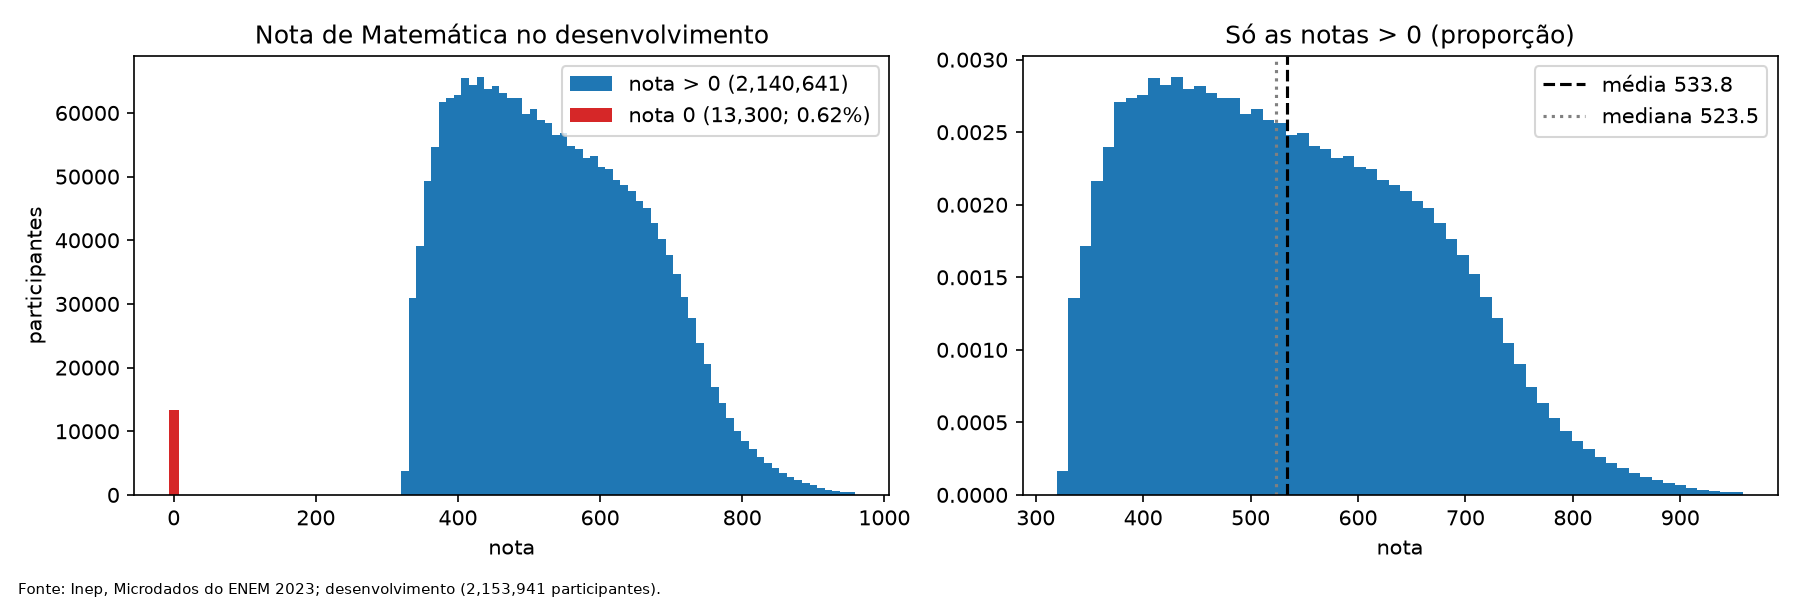
\includegraphics[width=0.9\textwidth,height=2.3in,keepaspectratio]{distribuicao_nota_dev.png}
\caption{Distribuição da nota de Matemática no desenvolvimento, com as notas zero em vermelho. Fonte: Inep, ENEM 2023; desenvolvimento (2.153.941 participantes).}
\end{figure*}

A nota tem média 533,8, mediana 523,5 e desvio padrão 131,6; as notas zero são 0,62\% do desenvolvimento e formam um pico isolado (Fig. 1). Prever sempre a média (baseline) erra 131,63 pontos de RMSE, o próprio desvio padrão. Na validação cruzada inicial (dataset de 30 colunas, Tabela I), o Gradient Boosting teve RMSE de 107,77 $\pm$ 0,23, contra 111,15 da regressão linear, e o stacking empatou com ele (107,76) a um custo cinco vezes maior; KNN (111,58) e SVR linear (111,15) não ganharam da regressão linear (Fig. 2). Dos sete modelos que passaram pela busca de hiperparâmetros, o bagging foi o que mais ganhou ($-$0,93) e o Gradient Boosting o que menos ($-$0,09, dentro do desvio de 0,18). Entre os oito datasets salvos (Tabela II), o melhor é o de 45 colunas (Gradient Boosting 107,05, 0,72 ponto melhor que o de 30): a escola dá o ganho mais consistente (cerca de 0,5), seguida de "não sei" e nacionalidade (0,2 a 0,4), e as três features criadas quase não mudam nada (0,01).

\begin{table*}[!t]
\caption{Configuração inicial de todos os modelos (validação cruzada, dataset de 30 colunas)}
\centering\footnotesize
\begin{tabularx}{\textwidth}{>{\raggedright\arraybackslash}Xcccc}
\toprule
\textbf{Modelo} & \textbf{RMSE ($\pm$ desvio)} & \textbf{MAE} & \textbf{R$^2$} & \textbf{Tempo/dobra (s)} \\
\midrule
Stacking & 107,76 $\pm$ 0,23 & 83,80 & 0,330 & 629,8 \\
Gradient Boosting & 107,77 $\pm$ 0,23 & 83,82 & 0,330 & 132,7 \\
Random Forest & 109,42 $\pm$ 0,19 & 85,49 & 0,309 & 103,4 \\
Pasting & 110,01 $\pm$ 0,21 & 86,00 & 0,302 & 19,8 \\
Bagging & 110,01 $\pm$ 0,21 & 85,99 & 0,302 & 24,1 \\
Árvore de decisão & 110,55 $\pm$ 0,19 & 86,38 & 0,295 & 3,0 \\
Ridge & 111,15 $\pm$ 0,18 & 86,96 & 0,287 & 0,3 \\
Regressão linear & 111,15 $\pm$ 0,18 & 86,96 & 0,287 & 0,7 \\
SVR linear & 111,15 $\pm$ 0,18 & 86,96 & 0,287 & 1,9 \\
KNN & 111,58 $\pm$ 0,18 & 87,18 & 0,282 & 476,3 \\
Baseline & 131,63 $\pm$ 0,16 & 107,58 & 0,000 & 0,1 \\
\bottomrule
\end{tabularx}
\\[2pt]{\scriptsize Fonte: Inep, ENEM 2023; validação cruzada no desenvolvimento.}
\end{table*}

\begin{table*}[!t]
\caption{RMSE médio por dataset salvo (validação cruzada, menor é melhor)}
\centering\footnotesize
\begin{tabularx}{\textwidth}{>{\raggedright\arraybackslash}Xcccc}
\toprule
\textbf{Dataset} & \textbf{Colunas} & \textbf{Regressão linear} & \textbf{Gradient Boosting (inicial)} & \textbf{Bagging otimizado} \\
\midrule
dataset\_1\_fundido & 30 & 111,15 & 107,77 & 109,08 \\
dataset\_1\_features & 33 & 111,15 & 107,76 & 109,17 \\
dataset\_2\_escola & 34 & 110,75 & 107,26 & 108,72 \\
dataset\_2\_features\_escola & 37 & 110,74 & 107,25 & 108,68 \\
dataset\_3\_sem\_escola & 38 & 110,75 & 107,55 & 109,09 \\
dataset\_3\_sem\_escola\_features & 41 & 110,74 & 107,54 & 109,08 \\
dataset\_3\_escola & 42 & 110,38 & 107,06 & 108,60 \\
\textbf{dataset\_3\_escola\_features} & \textbf{45} & \textbf{110,38} & \textbf{107,05} & \textbf{108,61} \\
\bottomrule
\end{tabularx}
\\[2pt]{\scriptsize Fonte: Inep, ENEM 2023; validação cruzada no desenvolvimento (notebook 02).}
\end{table*}

\textbf{Associação com a nota e os 21 conjuntos.} O Spearman \cite{spearman} de cada coluna com a nota (Tabela III) mostra a renda (Q006, +0,46) e os computadores em casa (Q024, +0,41) como as colunas mais associadas, seguidas da ocupação e da escolaridade dos responsáveis (+0,33 a +0,35) e de bens do domicílio (carros e banheiros, +0,34); língua estrangeira ($-$0,29), cor/raça ($-$0,22) e pessoas por quarto ($-$0,22) têm sinal negativo. Nenhuma coluna isolada passa de |$\rho$| = 0,46, e entre as colunas mantidas o maior valor é 0,63 (Q002 $\times$ Q004), abaixo do limite de 0,7; a fusão da trajetória escolar foi a única necessária. A Tabela IV lista os 21 conjuntos de entrada com o Gradient Boosting inicial: o melhor entre os salvos é o de 45 colunas (107,05), a UF dá o maior ganho entre as variações ($-$0,70) e retirar o bloco de perfil e trajetória o maior prejuízo (+4,42).

\begin{table*}[!t]
\caption{Spearman de colunas com a nota de Matemática (as 8 maiores e as 4 menores entre as 45 do dataset 3)}
\centering\footnotesize
\begin{tabularx}{\textwidth}{l>{\raggedright\arraybackslash}Xc}
\toprule
\textbf{Coluna} & \textbf{O que é} & \textbf{$\rho$ com a nota} \\
\midrule
Q006 & renda familiar mensal & +0,457 \\
Q024 & computadores em casa & +0,409 \\
Q003 & ocupação do pai ou responsável & +0,349 \\
Q002 & escolaridade da mãe ou responsável & +0,347 \\
Q004 & ocupação da mãe ou responsável & +0,346 \\
Q010 & carros & +0,339 \\
Q008 & banheiros & +0,339 \\
Q001 & escolaridade do pai ou responsável & +0,332 \\
Q001\_NAO\_SEI & indicador: não sabe a escolaridade do pai & $-$0,091 \\
PESSOAS\_POR\_QUARTO & criada: pessoas por quarto & $-$0,221 \\
TP\_COR\_RACA & cor/raça & $-$0,222 \\
TP\_LINGUA & língua estrangeira (inglês ou espanhol) & $-$0,287 \\
\bottomrule
\end{tabularx}
\\[2pt]{\scriptsize Fonte: Inep, ENEM 2023; 2.692.427 participantes com nota (notebook 01); tabela completa na documentação.}
\end{table*}

\begin{table*}[!t]
\caption{Os 21 conjuntos de entrada: Gradient Boosting inicial, validação cruzada}
\centering\footnotesize
\begin{tabularx}{\textwidth}{>{\raggedright\arraybackslash}Xccc}
\toprule
\textbf{Conjunto} & \textbf{Colunas} & \textbf{RMSE ($\pm$ desvio)} & \textbf{R$^2$} \\
\midrule
Salvo: dataset\_1\_fundido & 30 & 107,77 $\pm$ 0,23 & 0,330 \\
Salvo: dataset\_1\_features & 33 & 107,76 $\pm$ 0,24 & 0,330 \\
Salvo: dataset\_2\_escola & 34 & 107,26 $\pm$ 0,20 & 0,336 \\
Salvo: dataset\_2\_features\_escola & 37 & 107,26 $\pm$ 0,19 & 0,336 \\
Salvo: dataset\_3\_sem\_escola & 38 & 107,55 $\pm$ 0,21 & 0,332 \\
Salvo: dataset\_3\_sem\_escola\_features & 41 & 107,54 $\pm$ 0,22 & 0,333 \\
Salvo: dataset\_3\_escola & 42 & 107,06 $\pm$ 0,19 & 0,339 \\
Salvo: dataset\_3\_escola\_features & 45 & 107,05 $\pm$ 0,20 & 0,339 \\
Fusão da situação escolar, só treino & 48 & 107,05 $\pm$ 0,19 & 0,339 \\
Situação escolar em 4 colunas & 48 & 106,73 $\pm$ 0,19 & 0,343 \\
\textbf{4 colunas + UF (representação final)} & \textbf{74} & \textbf{106,02 $\pm$ 0,19} & \textbf{0,351} \\
Sem as 3 features criadas & 71 & 106,04 $\pm$ 0,17 & 0,351 \\
Seleção k = 22 & 22 de 74 & 110,61 $\pm$ 0,19 & 0,294 \\
Seleção k = 37 & 37 de 74 & 107,44 $\pm$ 0,21 & 0,334 \\
Seleção k = 51 & 51 de 74 & 107,07 $\pm$ 0,20 & 0,338 \\
Sem renda & 72 & 106,89 $\pm$ 0,19 & 0,341 \\
Sem escolaridade e ocupação dos responsáveis & 66 & 106,56 $\pm$ 0,17 & 0,345 \\
Sem bens e domicílio & 52 & 107,36 $\pm$ 0,17 & 0,335 \\
Sem escola & 70 & 106,44 $\pm$ 0,18 & 0,346 \\
Sem localização (UF) & 48 & 106,73 $\pm$ 0,19 & 0,343 \\
Sem perfil e trajetória & 62 & 110,45 $\pm$ 0,19 & 0,296 \\
\bottomrule
\end{tabularx}
\\[2pt]{\scriptsize Fonte: Inep, ENEM 2023; validação cruzada no desenvolvimento (8 salvos nos notebooks 01 e 02; 13 variações no notebook 04).}
\end{table*}

\begin{figure*}[!t]
\centering
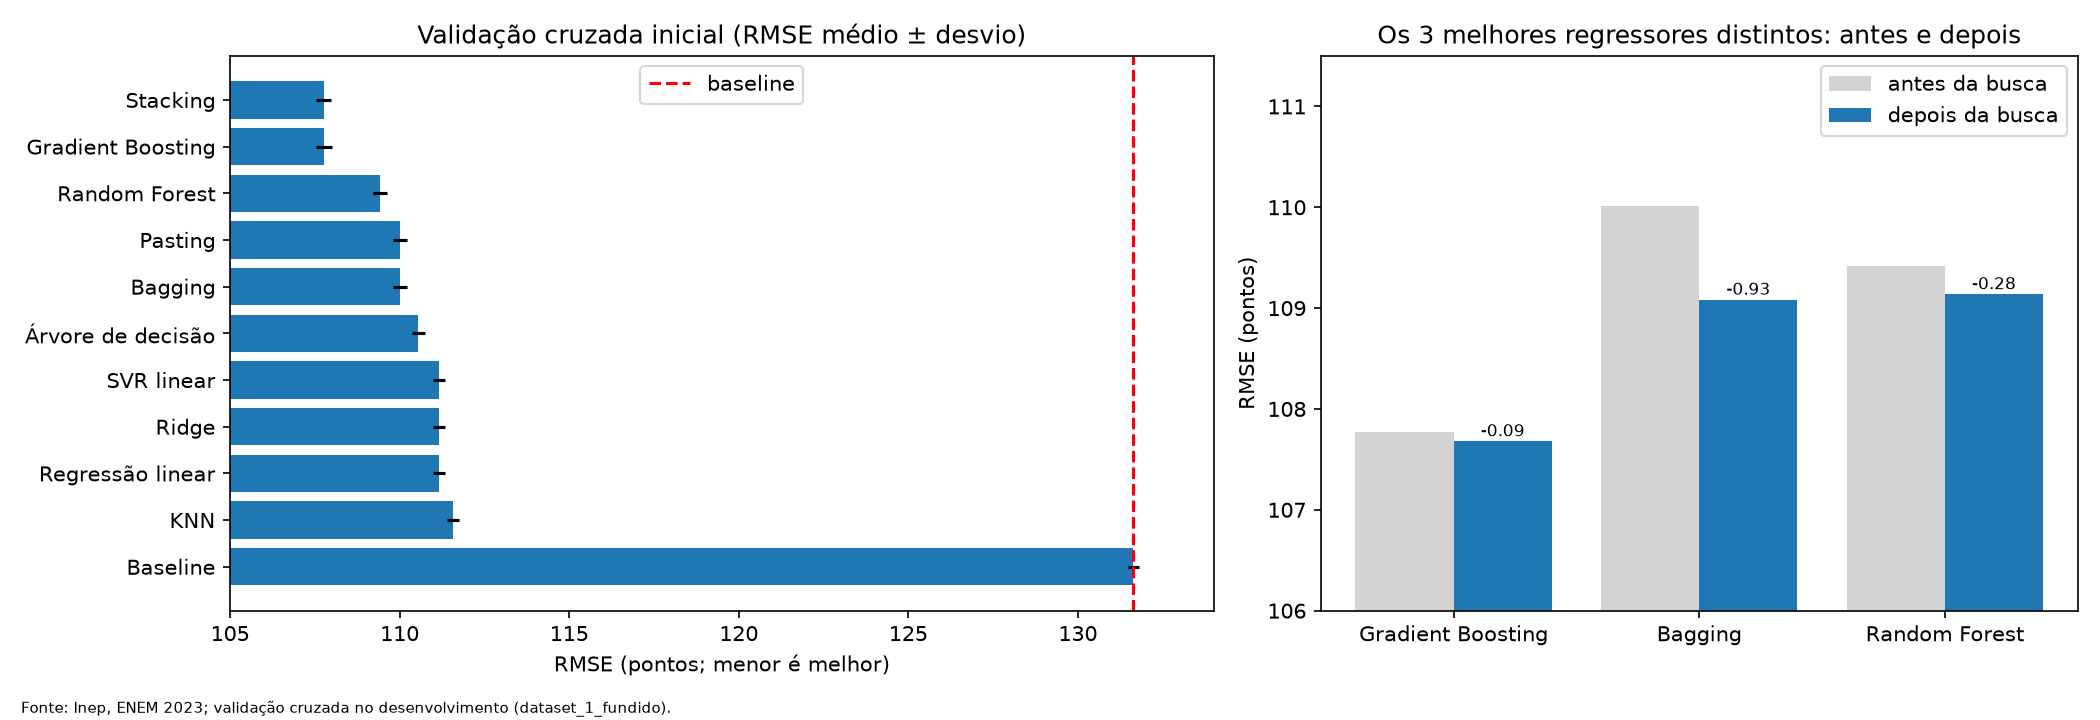
\includegraphics[width=0.9\textwidth,height=2.4in,keepaspectratio]{comparacao_modelos.png}
\caption{Validação cruzada inicial de todos os regressores contra o baseline (esquerda) e os três melhores regressores distintos antes e depois da busca (direita). Fonte: Inep, ENEM 2023; validação cruzada no desenvolvimento, dataset\_1\_fundido.}
\end{figure*}


\subsection{PCA}
Para atingir 80\% da variância explicada são necessários 18 de 30 componentes: os dados quase não se comprimem (Fig. 3). Dentro do Pipeline, o PCA piorou os dois regressores testados em todos os cortes: com 25 componentes, o RMSE do Gradient Boosting foi de 107,77 (sem PCA) para 110,17, e com 5 componentes para 113,21; na regressão linear, de 111,15 para 111,66 (25) e 114,43 (5). Nenhum corte ficou dentro de um desvio do modelo sem PCA. Como justificativa do número de componentes, 18 preservariam 80\% da variância, mas a decisão final foi não usar PCA.

\begin{figure*}[!t]
\centering
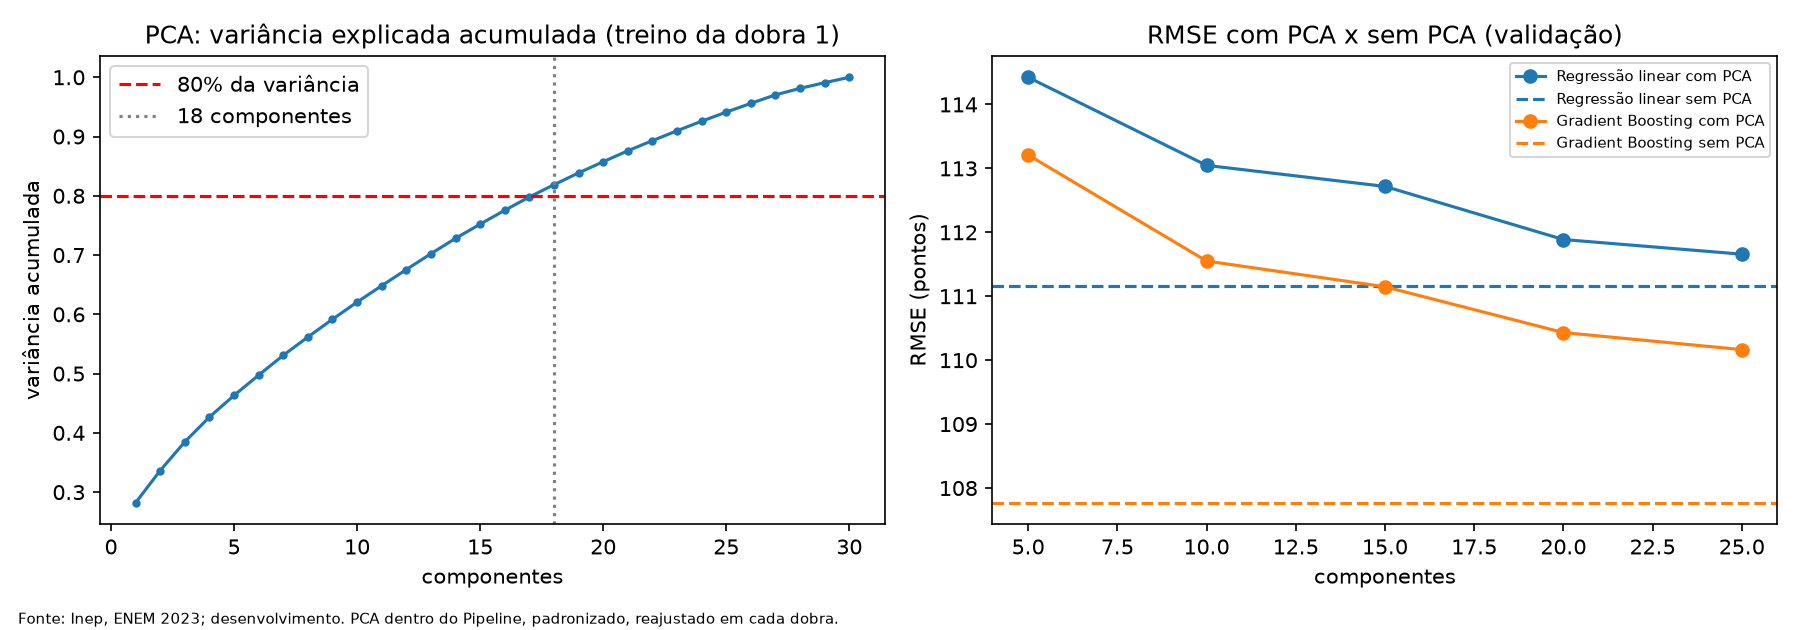
\includegraphics[width=0.9\textwidth,height=2.4in,keepaspectratio]{pca_variancia_e_rmse.png}
\caption{Variância explicada acumulada do PCA (esquerda; 18 componentes chegam a 80\%) e RMSE com e sem PCA em dois regressores (direita). Fonte: Inep, ENEM 2023; desenvolvimento. PCA padronizado e reajustado em cada dobra.}
\end{figure*}


\subsection{Hipóteses de preparação, seleção e balanceamento}
\begin{table*}[!t]
\caption{Hipóteses testadas (Gradient Boosting inicial, validação cruzada)}
\centering\footnotesize
\begin{tabularx}{\textwidth}{>{\raggedright\arraybackslash}Xcc}
\toprule
\textbf{Experimento} & \textbf{RMSE ($\pm$ desvio)} & \textbf{$\Delta$ RMSE} \\
\midrule
1a. Fusão da situação escolar, só treino & 107,051 $\pm$ 0,192 &  \\
1b. 4 colunas separadas & 106,726 $\pm$ 0,189 & -0,325 \\
2. 1b + UF da prova & 106,025 $\pm$ 0,188 & -0,701 \\
3. Sem as 3 features criadas & 106,038 $\pm$ 0,167 & +0,013 \\
4a. SelectKBest, k = 51 & 107,069 $\pm$ 0,199 & +1,044 \\
4b. SelectKBest, k = 22 & 110,607 $\pm$ 0,191 & +4,582 \\
5a. Pesos por faixa, $\alpha$ = 0,5 & 108,140 $\pm$ 0,188 & +2,115 \\
5b. Pesos por faixa, $\alpha$ = 1,0 & 123,459 $\pm$ 0,149 & +17,434 \\
6a. Sem perfil e trajetória & 110,445 $\pm$ 0,189 & +4,420 \\
6b. Sem bens e domicílio & 107,356 $\pm$ 0,174 & +1,331 \\
6c. Sem renda & 106,893 $\pm$ 0,194 & +0,868 \\
6d. Sem UF & 106,726 $\pm$ 0,189 & +0,701 \\
\bottomrule
\end{tabularx}
\\[2pt]{\scriptsize Fonte: Inep, ENEM 2023; desenvolvimento. $\Delta$ em relação à referência indicada (1a para 1b; 1b para 2; 2 para as demais).}
\end{table*}

\begin{figure*}[!t]
\centering
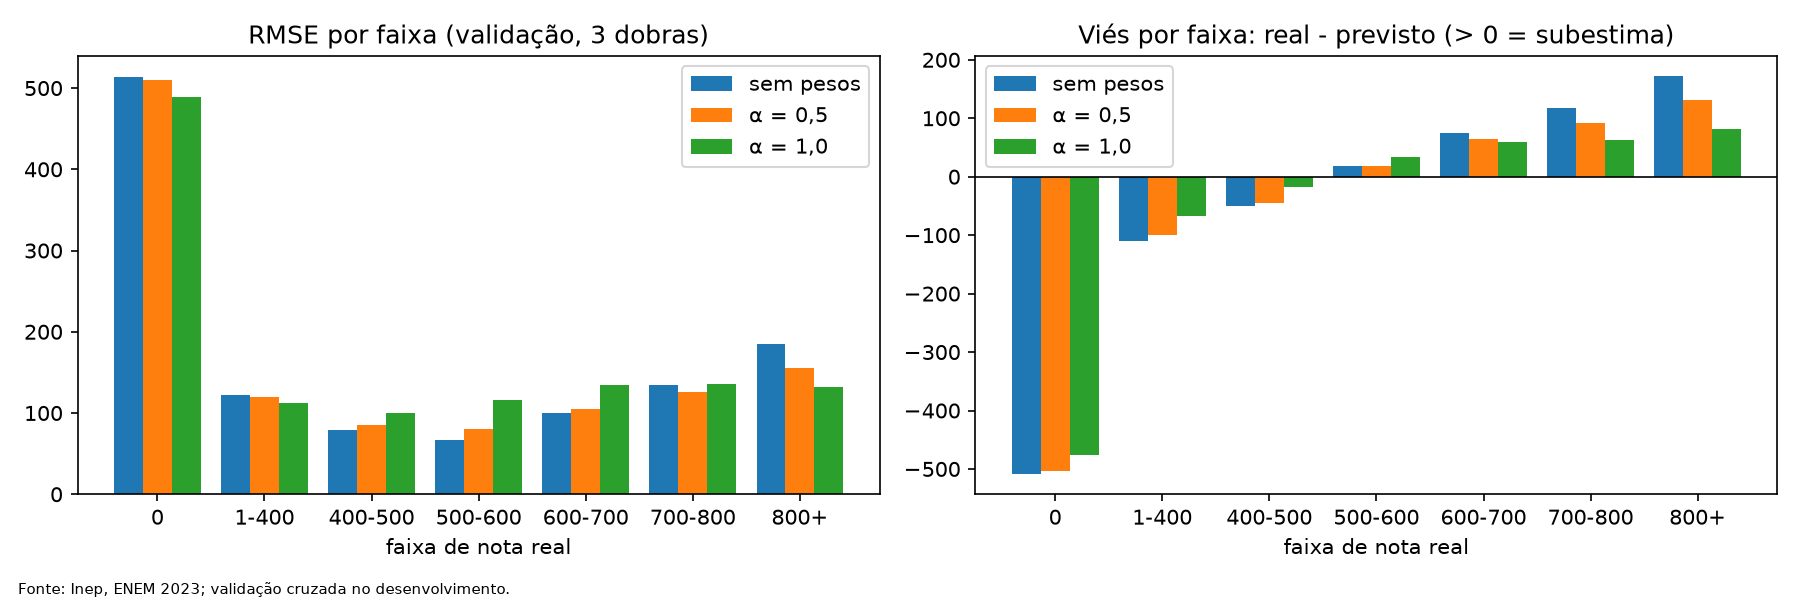
\includegraphics[width=0.9\textwidth,height=2.2in,keepaspectratio]{balanceamento_por_faixa.png}
\caption{RMSE e viés por faixa de nota real, sem pesos e com pesos $\alpha$ = 0,5 e $\alpha$ = 1,0. Fonte: Inep, ENEM 2023; validação cruzada no desenvolvimento.}
\end{figure*}

\begin{figure*}[!t]
\centering
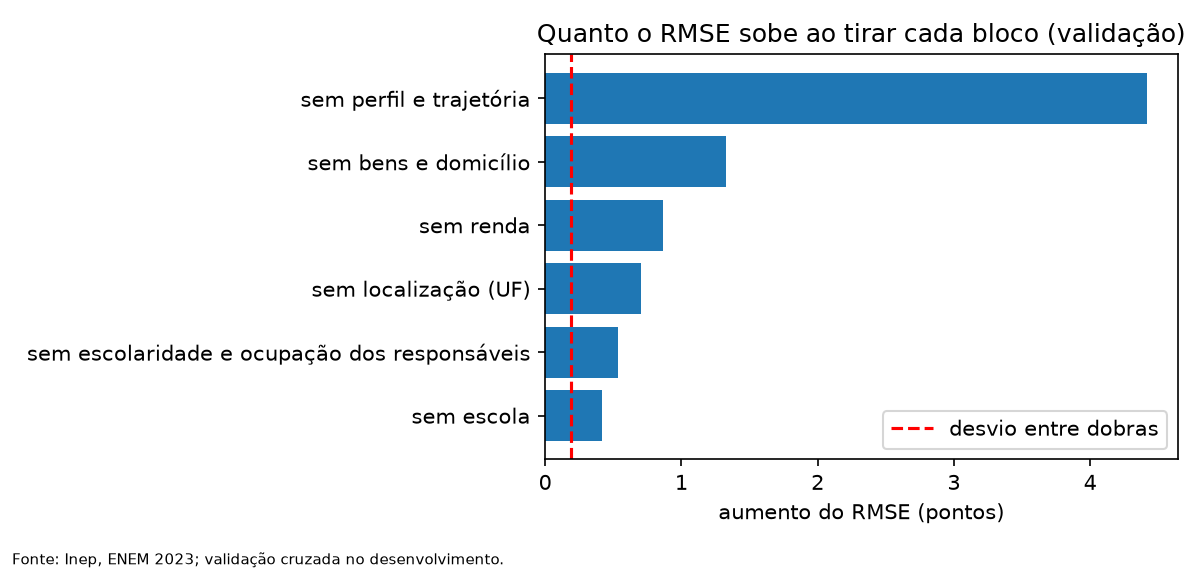
\includegraphics[width=0.9\textwidth,height=2.2in,keepaspectratio]{blocos_de_informacao.png}
\caption{Quanto o RMSE sobe ao retirar cada bloco de informação (linha vermelha: desvio entre dobras). Fonte: Inep, ENEM 2023; validação cruzada no desenvolvimento.}
\end{figure*}

A fusão das quatro colunas de trajetória, refeita só com o treino de cada dobra (RMSE 107,05; Tabela V), perdeu informação: mantê-las separadas deu 106,73 ($-$0,33), e acrescentar a UF da prova deu 106,03 ($-$0,70), ambas maiores que o desvio entre dobras (0,19). As três features criadas não tiveram efeito (+0,01). A seleção com SelectKBest piorou em todos os cortes (+1,04 com k = 51 e +4,58 com k = 22), então mantivemos as 74 colunas. A ponderação por faixa de nota piorou o RMSE geral (+2,12 e +17,43), mas reduziu o erro das notas altas: acima de 800 o RMSE caiu de 184,9 para 155,4 ($\alpha$ = 0,5) e 131,7 ($\alpha$ = 1,0) (Fig. 4), à custa das faixas do meio (de 66,8 para 80,6 na faixa de 500 a 600). Retirar um bloco de informação por vez piorou o erro em todos os casos; o bloco de perfil e trajetória pesa mais (+4,42), seguido de bens (+1,33), renda (+0,87) e UF (+0,70) (Fig. 5).


\subsection{Solução final e curva de aprendizado}
A solução final é o Gradient Boosting com os hiperparâmetros da busca, sobre 74 colunas (trajetória separada e UF), sem seleção, PCA nem pesos. Na validação cruzada teve RMSE de 105,86 $\pm$ 0,17 e R$^2$ de 0,353, contra 108,87 da regressão linear e 131,63 do baseline. Na curva de aprendizado (Fig. 6), de 10\% a 100\% do treino da dobra, o RMSE de treino sobe de 102,6 para 104,8 e o de validação cai de 106,7 para 105,9; a diferença encolhe de 4,1 para 1,1 ponto, e de 75\% para 100\% a validação melhora só 0,07 ponto, menos que o desvio entre dobras (0,2).

\begin{figure*}[!t]
\centering
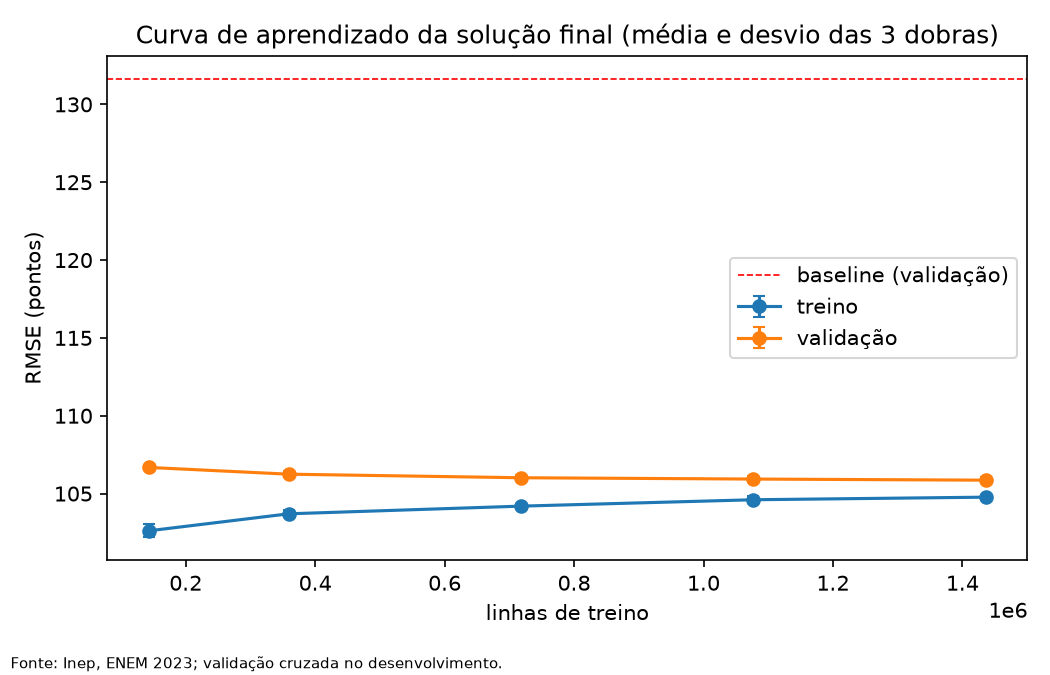
\includegraphics[width=0.9\textwidth,height=2.6in,keepaspectratio]{curva_aprendizado.png}
\caption{Curva de aprendizado da solução final: RMSE de treino e de validação (média e desvio das três dobras). Fonte: Inep, ENEM 2023; validação cruzada no desenvolvimento.}
\end{figure*}

\textbf{Importância das colunas.} A importância por permutação na validação da dobra 1 (5 mil pessoas, 3 repetições; Fig. 7) coloca no topo o ano de conclusão do ensino médio (+6,35 pontos de RMSE ao embaralhar a coluna), a renda familiar (Q006, +6,33) e a faixa etária (+5,59), seguidos de sexo (+2,29), língua estrangeira (+2,02) e computadores em casa (Q024, +1,53); cor/raça (+0,90) e escola privada (+0,80) vêm depois. As três primeiras tratam de trajetória e renda, o que concorda com o bloco que mais pesa na retirada (perfil e trajetória, +4,4). São associações, não causas, e colunas correlacionadas dividem a importância.

\begin{figure*}[!t]
\centering
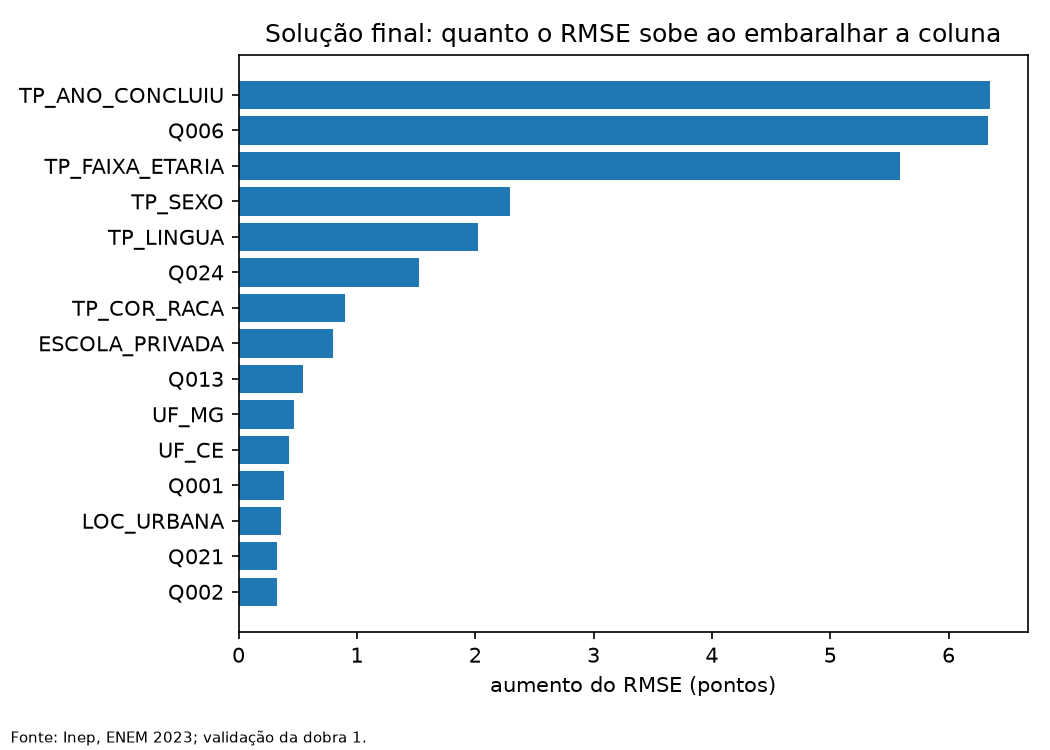
\includegraphics[width=0.9\textwidth,height=2.5in,keepaspectratio]{importancia_solucao_final.png}
\caption{Solução final: quanto o RMSE sobe ao embaralhar cada coluna (as 15 maiores), na validação da dobra 1. Fonte: Inep, ENEM 2023; validação cruzada no desenvolvimento.}
\end{figure*}


\subsection{Teste final}
O teste foi aberto uma única vez, com a solução fixada, nos 538.486 participantes reservados (Tabela VI). A solução final teve RMSE de 105,81, MAE de 82,00 e R$^2$ de 0,354, contra 131,70 do baseline e 108,86 da regressão linear sem regularização: 19,7\% menos erro que o baseline e 2,8\% menos que a regressão linear. O resultado de teste coincide com o da validação (105,81 contra 105,86), diferença menor que o desvio entre dobras.

\begin{table*}[!t]
\caption{Validação cruzada (média $\pm$ desvio) e teste do baseline, da regressão linear sem regularização e da solução final}
\centering\footnotesize
\begin{tabularx}{\textwidth}{>{\raggedright\arraybackslash}Xcccccccc}
\toprule
\textbf{Modelo} & \textbf{CV RMSE} & \textbf{CV MAE} & \textbf{CV R$^2$} & \textbf{CV s/dobra} & \textbf{Teste RMSE} & \textbf{Teste MAE} & \textbf{Teste R$^2$} & \textbf{Ajuste (s)} \\
\midrule
Baseline (média) & 131,63 $\pm$ 0,16 & 107,58 $\pm$ 0,06 & 0,000 & 0 & 131,70 & 107,64 & 0,000 & 0 \\
Regressão linear & 108,87 $\pm$ 0,16 & 84,86 $\pm$ 0,04 & 0,316 & 3 & 108,86 & 84,89 & 0,317 & 4 \\
\textbf{Solução final} & \textbf{105,86 $\pm$ 0,17} & \textbf{82,02 $\pm$ 0,05} & \textbf{0,353} & \textbf{91} & \textbf{105,81} & \textbf{82,00} & \textbf{0,354} & \textbf{165} \\
\bottomrule
\end{tabularx}
\\[2pt]{\scriptsize Fonte: Inep, ENEM 2023; validação cruzada no desenvolvimento e teste (538.486 participantes).}
\end{table*}

Os resíduos têm média 0,1 e desvio 105,8, e a média do resíduo fica perto de zero em toda a faixa prevista. As previsões ficam concentradas entre cerca de 350 e 850, enquanto as notas reais vão de 0 a 1000 (regressão à média, Fig. 8); as notas zero formam uma faixa isolada de resíduos entre $-$370 e $-$770. O erro é mínimo perto da média (RMSE 67 na faixa de 500 a 600) e cresce nas pontas com viés de sinal oposto: +171 pontos acima de 800 (11.243 participantes) e $-$510 nos zeros (3.338) (Fig. 9). Nos grupos de região, renda, escola e sexo o viés médio é menor que 1 ponto (por UF, até 2,5); o RMSE vai de 97,3 (renda até 1 salário, 187.962 participantes) a 113,3 (renda de 6 a 10 salários, 34.469) e de 97,9 (região Norte, 57.603) a 111,0 (Sul, 58.227), com R$^2$ dentro de cada faixa de renda entre 0,17 e 0,21: o erro maior nos grupos de renda alta acompanha uma nota mais dispersa, não um modelo pior para eles.

\begin{figure*}[!t]
\centering
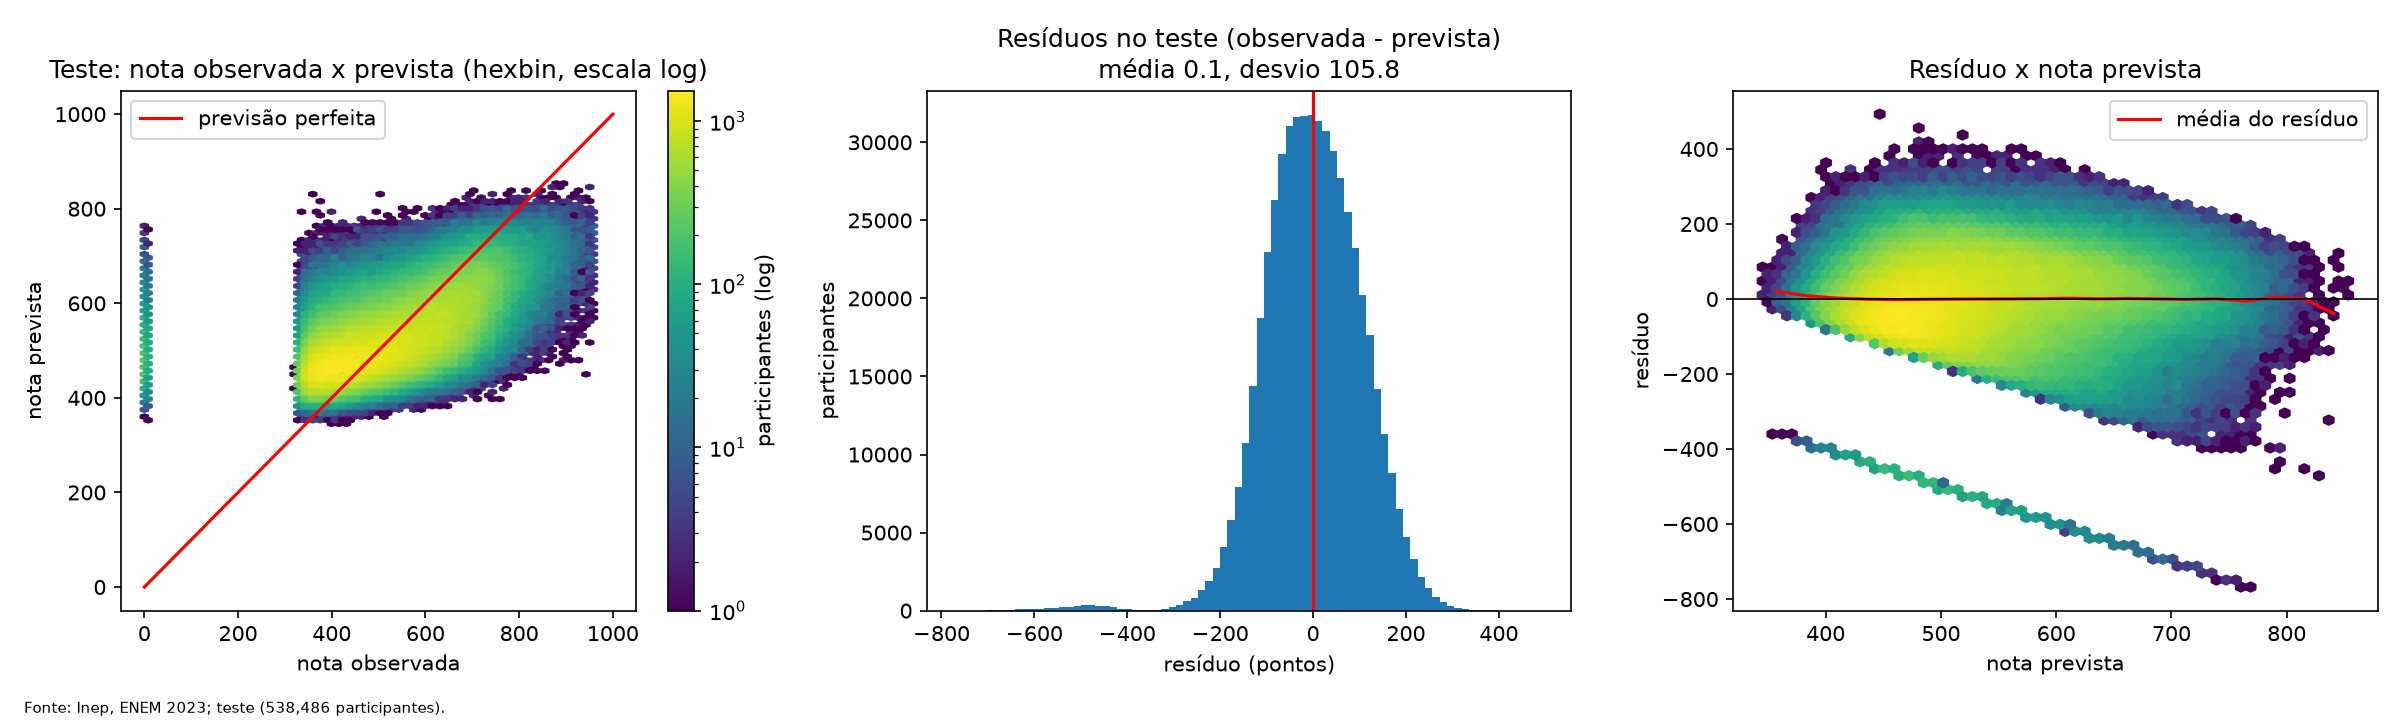
\includegraphics[width=0.9\textwidth,height=2.2in,keepaspectratio]{teste_real_previsto_residuos.png}
\caption{Teste: nota observada contra prevista (a reta vermelha é a previsão perfeita), histograma dos resíduos e resíduo contra nota prevista. Fonte: Inep, ENEM 2023; teste (538.486 participantes); dispersão agregada em células hexagonais.}
\end{figure*}

\begin{figure*}[!t]
\centering
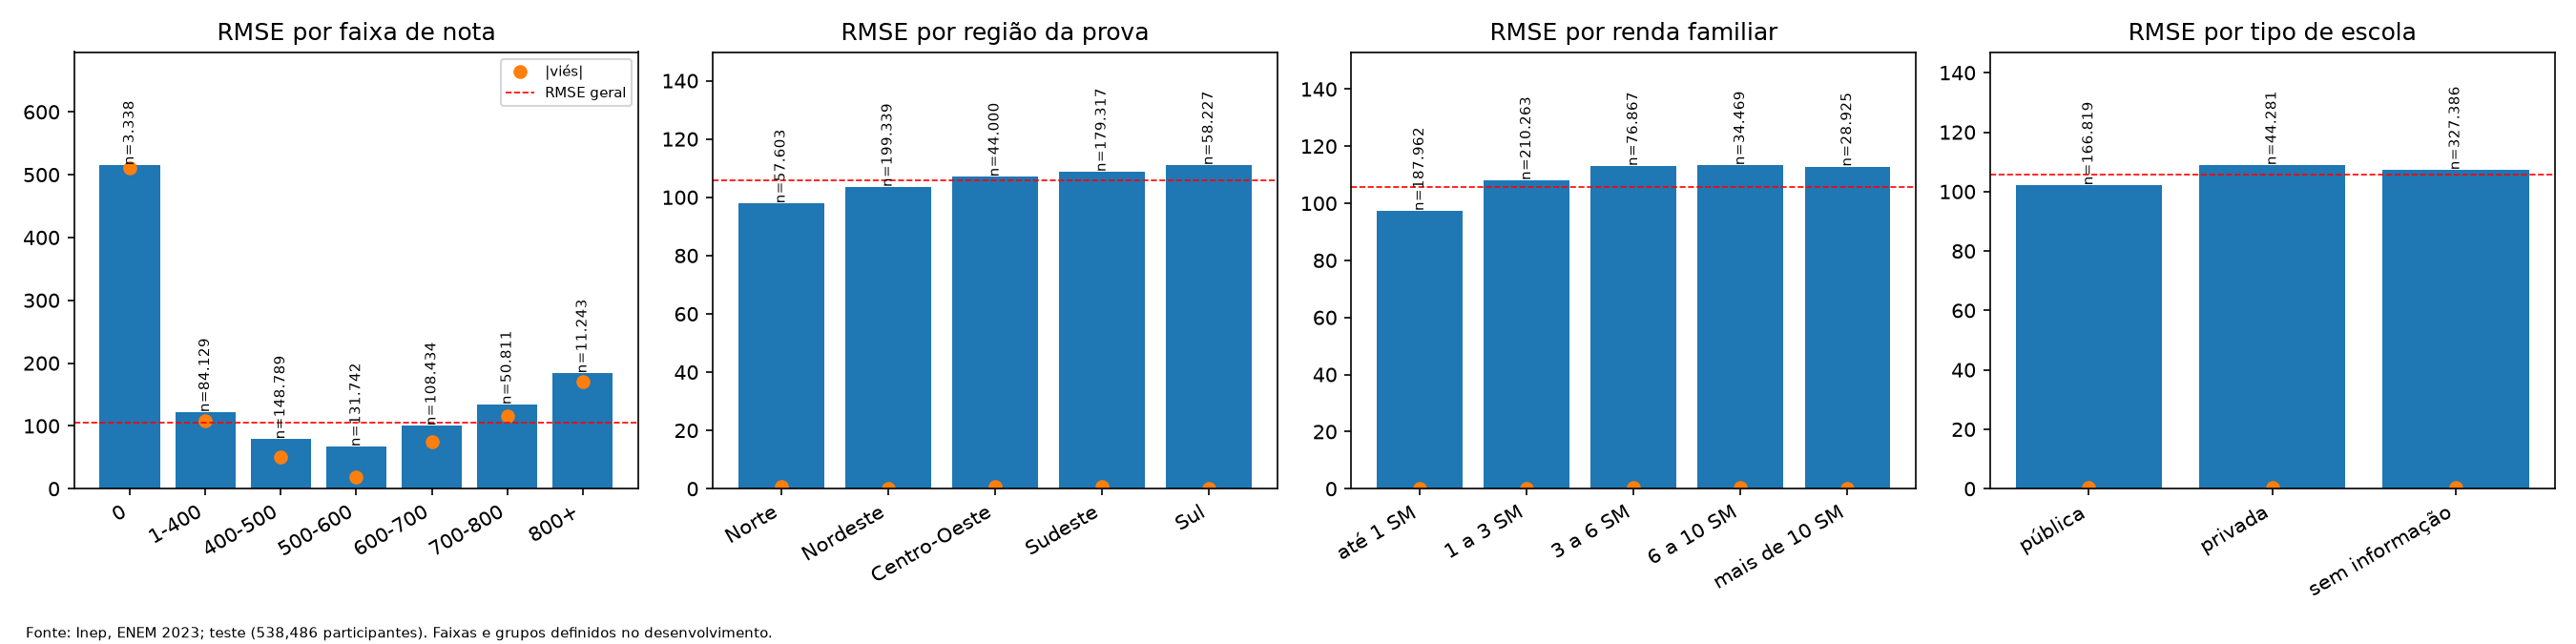
\includegraphics[width=0.9\textwidth,height=2.0in,keepaspectratio]{teste_erros_por_faixa_e_grupo.png}
\caption{Teste: RMSE por faixa de nota, região da prova, faixa de renda e tipo de escola, com o tamanho de cada grupo. Fonte: Inep, ENEM 2023; teste; faixas e grupos definidos no desenvolvimento.}
\end{figure*}


\subsection{Solução independente de outra IA (dataset 5)}
A solução independente, no mesmo teste de 538.486 participantes, teve como melhor modelo o Ridge com one-hot de todas as categóricas (RMSE 107,53), seguido do SVR linear (107,89), do Gradient Boosting leve de 50 árvores (108,07) e da Random Forest de 30 árvores (108,13) (Tabela VII). Nenhum supera a nossa solução final (105,81). O ganho dela aparece nos modelos lineares: o Ridge com one-hot erra 1,33 ponto a menos que a nossa regressão linear sem regularização (108,86), o que confirma que tratar cor/raça, estado civil e as escadas do questionário como números prejudica o modelo linear; já a regressão linear sem regularização dela (109,70) fica pior que a nossa, então o ganho vem do one-hot somado à regularização. Como ela não fez validação cruzada, a comparação do teste é só descritiva e nada foi escolhido a partir dela; reproduzimos a preparação dela e a avaliamos nas nossas dobras (Seção III-H), com o mesmo resultado.

\begin{table*}[!t]
\caption{Teste: solução independente (dataset 5) contra a nossa}
\centering\footnotesize
\begin{tabularx}{\textwidth}{>{\raggedright\arraybackslash}Xccc}
\toprule
\textbf{Modelo} & \textbf{RMSE} & \textbf{MAE} & \textbf{R$^2$} \\
\midrule
\textbf{Nossa solução final (Gradient Boosting, 74 colunas)} & \textbf{105,81} & \textbf{82,00} & \textbf{0,354} \\
Dataset 5: Ridge & 107,53 & 83,63 & 0,333 \\
Dataset 5: SVR linear & 107,89 & 83,30 & 0,329 \\
Dataset 5: Gradient Boosting (50 árvores) & 108,07 & 84,46 & 0,327 \\
Dataset 5: Random Forest (30 árvores) & 108,13 & 84,32 & 0,326 \\
Nossa regressão linear sem regularização & 108,86 & 84,89 & 0,317 \\
Dataset 5: regressão linear & 109,70 & 84,05 & 0,306 \\
Baseline (média) & 131,70 & 107,64 & 0,000 \\
\bottomrule
\end{tabularx}
\\[2pt]{\scriptsize Fonte: Inep, ENEM 2023; teste (538.486 participantes), linhas de árvore, bagging, pasting e AdaBoost do dataset 5 omitidas.}
\end{table*}


\subsection{Diagnóstico com as notas de outras áreas (dataset 6)}
Este diagnóstico \textbf{não faz parte da solução}: as notas de outras áreas são proibidas como entrada e foram usadas só para medir o vazamento, por validação cruzada no desenvolvimento, sem abrir o teste. Entre as colunas do dataset 6, as quatro notas são as mais associadas à nota de Matemática pelo Spearman: Humanas 0,66, Linguagens 0,64, Natureza 0,64 e Redação 0,53, contra 0,46 da renda; Humanas e Linguagens passam do limite de redundância entre si (0,79), e as três colunas de ausência do primeiro dia são idênticas ($\rho$ = 1). Com as quatro notas o RMSE do Gradient Boosting cai de 107,05 para 74,43 e o R$^2$ sobe de 0,339 para 0,680; só com a Natureza, a prova do mesmo dia, o RMSE já é 82,83 (Tabela VIII, Fig. 10). Mesmo com o vazamento o R$^2$ não chega a 1: cerca de um terço da nota continua sem explicação. As notas zero deixam de ser ruído quando essas notas entram: 98,3\% de quem zerou Matemática também tem 0 em Natureza, e tirar os zeros do treino piora o erro geral (RMSE de 74,43 para 82,81), porque o modelo passa a prever cerca de 470 para eles (RMSE de 471 nos zeros, contra 69 com eles no treino). Só com o perfil, tirar os zeros não muda nada (107,05 contra 107,12).

\begin{table*}[!t]
\caption{Diagnóstico com vazamento (dataset 6, fora da solução): validação cruzada}
\centering\footnotesize
\begin{tabularx}{\textwidth}{>{\raggedright\arraybackslash}Xccc}
\toprule
\textbf{Entrada} & \textbf{Gradient Boosting: RMSE} & \textbf{R$^2$} & \textbf{Regressão linear: RMSE} \\
\midrule
Só o perfil (45 colunas) & 107,05 $\pm$ 0,20 & 0,339 & 110,38 \\
+ Natureza (mesmo dia) & 82,83 $\pm$ 0,06 & 0,604 & 86,05 \\
+ Humanas, Linguagens e Redação (dia 1) & 85,96 $\pm$ 0,23 & 0,574 & 89,69 \\
\textbf{+ as quatro notas} & \textbf{74,43 $\pm$ 0,03} & \textbf{0,680} & \textbf{79,63} \\
+ as quatro notas, sem zeros no treino & 82,81 $\pm$ 0,14 & 0,604 & 80,51 \\
\bottomrule
\end{tabularx}
\\[2pt]{\scriptsize Fonte: Inep, ENEM 2023; validação cruzada no desenvolvimento. Última linha: Gradient Boosting e regressão linear com zeros fora do treino.}
\end{table*}

\begin{figure*}[!t]
\centering
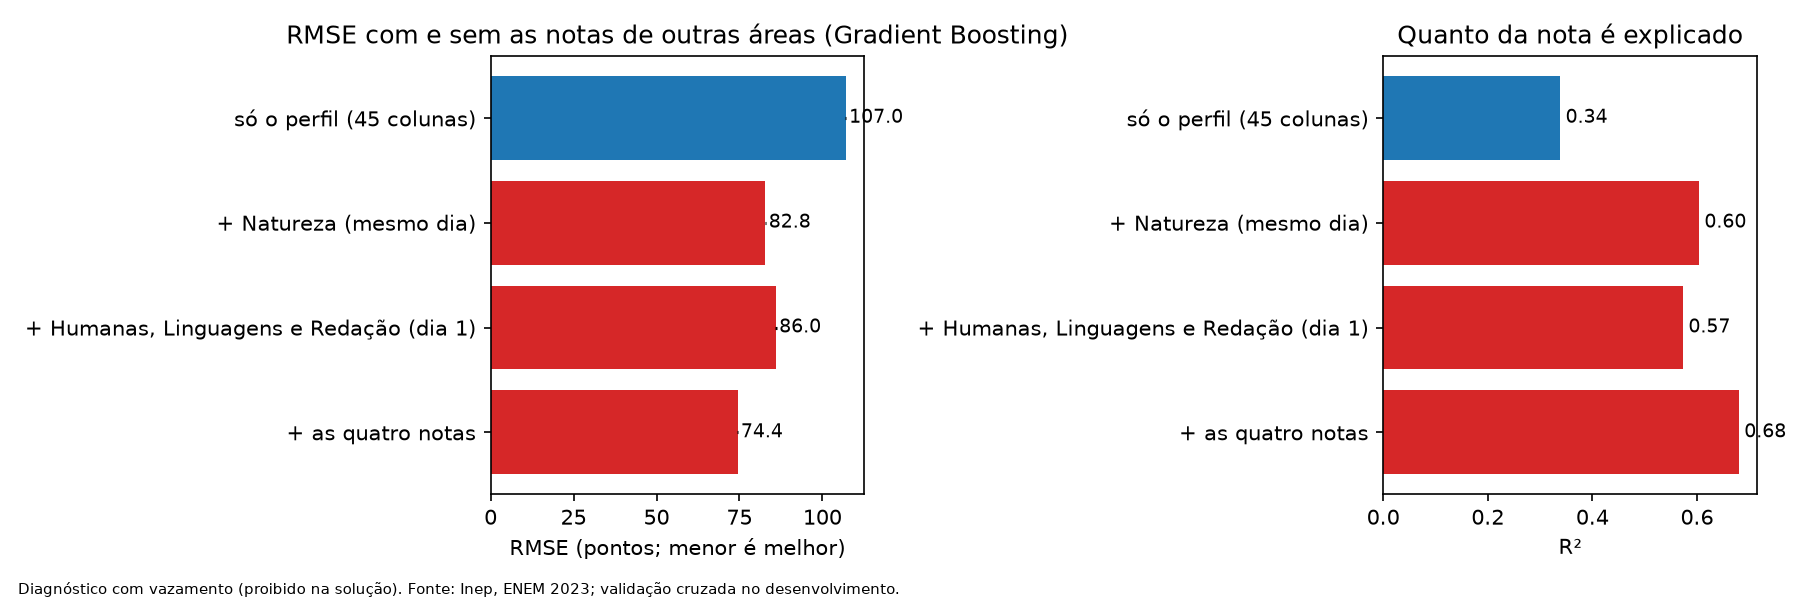
\includegraphics[width=0.9\textwidth,height=2.2in,keepaspectratio]{diagnostico_dataset6.png}
\caption{Diagnóstico com vazamento (dataset 6, fora da solução): RMSE e R$^2$ do Gradient Boosting só com o perfil e com as notas de outras áreas. Fonte: Inep, ENEM 2023; validação cruzada no desenvolvimento.}
\end{figure*}


\subsection{Extensões após o teste (só validação cruzada)}
Como o teste já havia sido aberto, estas hipóteses extras não alteram a solução final; foram medidas nas mesmas três dobras do desenvolvimento (Tabela IX). (i) One-hot em todas as categóricas reduz o RMSE da regressão linear de 108,87 para 107,89 (só nas colunas nominais, 0,24), o ganho de cerca de 1 ponto que a solução independente sugeria; mesmo assim, fica 2 pontos atrás do Gradient Boosting. (ii) O V de Cramér entre as nove colunas sem ordem passa de 0,7 só para situação de conclusão e tipo de escola (0,707), par já tratado pela fusão. (iii) O município com target encoding dentro do Pipeline melhora 0,30 ponto (106,03 para 105,73) nas três dobras, mais que o desvio entre dobras (0,19); contra a solução final, o ganho cai para 0,13. (iv) Quatro sementes dão RMSE de 105,862 a 105,871, variação de 0,009. (v) A busca de hiperparâmetros nas 74 colunas finais reencontra o mesmo erro (105,859 contra 105,864). (vi) A preparação do dataset 5 avaliada nas nossas dobras dá 107,51 com Ridge, igual à métrica de teste dela (107,5), e fica 1,6 ponto acima da nossa solução (105,86).

\begin{table*}[!t]
\caption{Extensões após o teste: validação cruzada no desenvolvimento}
\centering\footnotesize
\begin{tabularx}{\textwidth}{>{\raggedright\arraybackslash}Xcc}
\toprule
\textbf{Experimento} & \textbf{RMSE médio $\pm$ desvio} & \textbf{R$^2$} \\
\midrule
Linear, tudo como número & 108,87 $\pm$ 0,16 & 0,316 \\
Linear, one-hot em todas as categóricas & 107,89 $\pm$ 0,18 & 0,328 \\
Gradient Boosting sem município (74 colunas) & 106,03 $\pm$ 0,19 & 0,351 \\
\textbf{Gradient Boosting com município (target encoding)} & \textbf{105,73 $\pm$ 0,17} & \textbf{0,355} \\
Solução final, sementes 42 / 0 / 1 / 2 & 105,86 / 105,86 / 105,87 / 105,87 & 0,353 \\
Busca nas 74 colunas: Gradient Boosting & 105,86 $\pm$ 0,18 & 0,353 \\
Dataset 5 por validação cruzada: Ridge & 107,51 $\pm$ 0,20 & 0,333 \\
\bottomrule
\end{tabularx}
\\[2pt]{\scriptsize Fonte: Inep, ENEM 2023; 3 dobras do desenvolvimento; teste não utilizado.}
\end{table*}


\subsection{As perguntas de investigação e as respostas}
Cada teste respondeu a uma pergunta. As oito primeiras vêm das perguntas de aprofundamento do enunciado; as duas últimas surgiram dos resultados (Tabela X). Ficaram de fora os dados externos, os modelos regionais e a transformação do alvo ou da perda.

\begin{table*}[!t]
\caption{Perguntas de investigação e respostas (RMSE médio, validação cruzada)}
\centering\footnotesize
\begin{tabularx}{\textwidth}{l>{\raggedright\arraybackslash}X}
\toprule
\textbf{Pergunta} & \textbf{Resposta} \\
\midrule
1. Quais blocos de informação contribuem mais? & Perfil e trajetória (+4,42), bens (+1,33) e renda (+0,87) são os que mais fazem falta. \\
2. O tratamento das categorias faz diferença? & Situação escolar separada: $-$0,33; "não sei" com indicador: cerca de $-$0,2; one-hot em modelos lineares: $-$0,98. \\
3. As interações ajudam? & Não: retirar as três features criadas muda o erro em +0,01. \\
4. A localização acrescenta informação? & Sim, pouco: UF $-$0,70; município $-$0,30 (depois do teste, não adotado). \\
5. Dados externos melhoram o contexto? & Não testado. \\
6. Existem perfis semelhantes? & K-means como feature: 107,79 contra 107,77, sem diferença. \\
7. Dá para reduzir os erros nas notas extremas? & Pesos por faixa: acima de 800, 185 para 155, mas +2,1 no erro geral; sem os zeros no treino, sem diferença. \\
8. Uma solução mais simples mantém o desempenho? & Não: seleção piora em 1,0 a 4,6, PCA piora, e a regressão linear perde 3,0 (30 vezes mais rápida). \\
9. Alguém sem contexto chegaria a algo melhor? & Não: 107,53 no teste e 107,51 por validação cruzada, contra 105,81 e 105,86. \\
10. O limite vem da informação ou do modelo? & Da informação: treino e validação a 1,1 ponto; com as notas de outras áreas, o R$^2$ vai de 0,34 a 0,68. \\
\bottomrule
\end{tabularx}
\\[2pt]{\scriptsize Fonte: Inep, ENEM 2023; ids dos experimentos e seções no relatório detalhado (documentação do repositório).}
\end{table*}


\section{Discussão}
\textbf{Limite de informação.} Famílias muito diferentes (linear, árvores, KNN, bagging e boosting) terminam num intervalo estreito de RMSE (106 a 112), e as árvores só ganham de três a quatro pontos da regressão linear. A curva de aprendizado mostra treino e validação separados por apenas 1,1 ponto e sem ganho relevante com mais dados, o que não indica sobreajuste forte. Erros altos e próximos podem ser subajuste, mas também falta de informação; aqui, a convergência de modelos tão distintos e o ganho mínimo do Gradient Boosting com 500 árvores sobre o inicial ($-$0,16) sugerem que a variação restante vem do que o perfil não captura (esforço de estudo, qualidade do ensino, circunstâncias do dia da prova), e não da falta de capacidade do modelo. Isso é uma interpretação, não um resultado medido.

\textbf{Desempenho e complexidade.} O ganho de 3 pontos de RMSE do Gradient Boosting sobre a regressão linear custa cerca de 30 vezes mais tempo por dobra (91 s contra 3 s). O stacking não ganhou do Gradient Boosting e custou cinco vezes mais. A seleção de atributos e o PCA reduzem colunas, mas pioram o erro em 1 a 5 pontos; a solução mais simples que preservou o erro foi manter todas as colunas e deixar o modelo de árvores escolher. As três features criadas, calculadas a partir de colunas já presentes, não acrescentaram informação a esse modelo.

\textbf{Erros nas pontas e grupos.} O modelo regride à média: superestima as notas baixas e subestima as altas. A ponderação mostra um compromisso explícito entre o erro das pontas e o das faixas do meio, onde está quase toda a população; a escolha depende do objetivo (identificar notas altas ou minimizar o erro médio). O viés médio por região, renda, escola e sexo é próximo de zero, mas as associações (renda, escola, idade) não indicam causa nem a capacidade de uma pessoa, e com erro médio de cerca de 82 pontos o modelo não serve para decisões individuais.

\textbf{Replicação e diagnóstico.} A solução independente de outra IA, com outro tratamento das categorias, chegou a um patamar parecido (107,5 a 108,1 contra 105,8) sem busca nem validação cruzada, o que reforça que o resultado não depende de uma escolha de preparação específica; o ganho dela, restrito aos modelos lineares, vem do one-hot. O diagnóstico com as notas de outras áreas mostra o outro lado: com informação sobre a própria prova o R$^2$ dobra (0,34 para 0,68), então o limite de cerca de 0,35 vem do que o perfil descreve, e não do algoritmo. Isso não autoriza usar essas notas, que só existem depois da prova e respondem a outra pergunta; e mesmo com elas sobra cerca de um terço da variação sem explicação.

\textbf{Limitações.} A divisão avalia novos participantes da mesma edição, não escolas ou municípios inéditos; UF e escola não são residência. Os hiperparâmetros foram buscados no dataset de 30 colunas e reaproveitados na representação final (uma busca nova nas 74 colunas deu o mesmo erro); stacking e KNN não passaram pela busca por custo. Cor/raça e estado civil entram como números em escada, o que as árvores toleram e a regressão linear não; o município (cerca de 1.750 categorias) não entrou na solução final; com target encoding melhorou 0,13 a 0,30 ponto, mas só depois de o teste ser aberto. A solução final usa a semente 42, e outras três sementes variaram 0,009 ponto, bem menos que o desvio entre dobras. Um vazamento pequeno nos datasets iniciais (média e desvio da fusão com todas as linhas) foi medido em 0,003 ponto de RMSE e corrigido no Pipeline final.


\section{Conclusão}
O perfil socioeconômico, escolar e demográfico permite estimar a nota de Matemática do ENEM 2023 apenas de forma aproximada: a solução final erra 105,81 pontos de RMSE no teste e explica 0,354 da variação, contra 131,70 do baseline. O que mais ajudou foi usar um modelo de árvores, manter a trajetória escolar sem fusão e incluir a UF; PCA, seleção de atributos, features combinadas, retirada dos zeros e K-means não ajudaram, e a ponderação troca erro das notas altas por erro das médias. A concordância entre validação e teste, e a curva de aprendizado, indicam que o limite é a informação disponível. Uma solução independente de outra IA, no mesmo teste, ficou em 107,5 e um diagnóstico com as notas de outras áreas (proibidas na solução) elevou o R$^2$ a 0,68, ambos coerentes com esse limite. Como próximo passo, o município com codificação supervisionada dentro do Pipeline, que já mostrou ganho pequeno (0,3 ponto) na validação cruzada.


\begin{thebibliography}{99}
\bibitem{inep} Inep, "Microdados do ENEM 2023 e dicionário de variáveis," Instituto Nacional de Estudos e Pesquisas Educacionais Anísio Teixeira, Brasília, DF, 2024. [Online]. Disponível: \url{https://www.gov.br/inep/pt-br/acesso-a-informacao/dados-abertos/microdados/enem}
\bibitem{spearman} C. Spearman, "The proof and measurement of association between two things," \textit{Am. J. Psychol.}, vol. 15, no. 1, pp. 72--101, 1904.
\bibitem{hoerl} A. E. Hoerl and R. W. Kennard, "Ridge regression: Biased estimation for nonorthogonal problems," \textit{Technometrics}, vol. 12, no. 1, pp. 55--67, 1970.
\bibitem{breiman96} L. Breiman, "Bagging predictors," \textit{Mach. Learn.}, vol. 24, no. 2, pp. 123--140, 1996.
\bibitem{breiman01} L. Breiman, "Random forests," \textit{Mach. Learn.}, vol. 45, no. 1, pp. 5--32, 2001.
\bibitem{friedman} J. H. Friedman, "Greedy function approximation: A gradient boosting machine," \textit{Ann. Statist.}, vol. 29, no. 5, pp. 1189--1232, 2001.
\bibitem{wolpert} D. H. Wolpert, "Stacked generalization," \textit{Neural Netw.}, vol. 5, no. 2, pp. 241--259, 1992.
\bibitem{sklearn} F. Pedregosa et al., "Scikit-learn: Machine learning in Python," \textit{J. Mach. Learn. Res.}, vol. 12, pp. 2825--2830, 2011.
\bibitem{jolliffe} I. T. Jolliffe, \textit{Principal Component Analysis}, 2nd ed. New York, NY, USA: Springer, 2002.
\bibitem{bergstra} J. Bergstra and Y. Bengio, "Random search for hyper-parameter optimization," \textit{J. Mach. Learn. Res.}, vol. 13, pp. 281--305, 2012.
\bibitem{ke} G. Ke et al., "LightGBM: A highly efficient gradient boosting decision tree," in \textit{Proc. Adv. Neural Inf. Process. Syst. (NIPS)}, 2017, pp. 3146--3154.
\bibitem{skdoc} scikit-learn developers, "User guide: Cross-validation, pipelines, model evaluation and ensembles." [Online]. Disponível: \url{https://scikit-learn.org/stable/user_guide.html}
\end{thebibliography}

\end{document}
